\usepackage[english]{babel}
\mode<article>{
  \usepackage{caption}
  \usepackage{subcaption}
}
\usepackage{hyperref}
\usepackage{listings}
\lstdefinelanguage{screensession}{
  basicstyle=\color{black}\ttfamily\small,
  basewidth=0.45em,
  numbers=left,
  numberstyle=\tiny\color{lightgray},
  delim=**[il][\color{gray}\$ \color{blue}]{>>\ }
}

\title{Git Concepts}
\author{Daniel Ruoso, Scott Lee}
\begin{document}
\mode<all>{\lstset{language=screensession}}

\maketitle
\begin{frame}<presentation>
  \titlepage
\end{frame}

\begin{abstract}
  This is the handout material for the Git Concepts training class. It
  covers the essential concepts of Git, some basic commands and then points to
  where you can find more learning resources.
\end{abstract}

\section{Introduction}

This class covers the concepts that are essential to understanding
Git.  It is not a tutorial in the sense that it does not focus on
``how to use Git''.  There are several documents of that nature on
the Internet. The intent is to prepare you to understand the Git
documentation and tutorials because many of them fail to present
these essential concepts, making them difficult to use by the
beginner.

This will not cover all Git commands or specific details of syntax.
There are examples, but just enough to make the concepts concrete
and understandable. This document is not intended as a Git reference
guide.

\begin{frame}[fragile]
  \label{WhatIsCovered}
  \frametitle{What is covered}

  \only<2>{
    \begin{itemize}
    \item Heavy focus on concepts
    \item Basic commands
    \item Where to learn more
    \end{itemize}
  }

  \note{
    \begin{itemize}
    \item Not a step-by-step tutorial
    \item Will not cover all Git commands
    \item Concepts required to understand documentation
    \end{itemize}
  }
\end{frame}

It is assumed that you have a basic understand of version control,
such as
what a ``working copy'' is and how it contrasts with a ``repository''
and the process of ``check in'' and ``check out''.
We also expect that you have some understanding of ``branches''
and ``merge'' operations. If you don't understand
what these are, stop now and do some research before continuing.

\begin{frame}[fragile]
  \label{ThingsWeAssumeYouKnow}
  \frametitle{Things we assume you know}

  \only<2>{
    \begin{itemize}
    \item Working copy
    \item Repository
    \item Check in/check out
    \item Branch
    \item Merge
    \end{itemize}
  }

  \note{ Explaining these concepts would require an entire class on its
    own, so we assume the audience has some experience with version
    control systems.}

\end{frame}

In section \ref{GitOverview} we will start by introducing what Git is,
its advantages and the basic operations. Later on in
section \ref{GitConcepts} we will go through the concepts behind the
way Git works. More information on how to get help on Git can be found
in section \ref{GitHelp}.

\section{Git Overview}
\label{GitOverview}

Git is a Decentralized Version Control System, which means that
instead of just creating a local working copy for the files managed by
the repository, you get a stand alone copy of the entire
repository. This means you can create local branches to work on
experimental code that might never be published while you still have
all the version control features.

\begin{frame}[fragile]
  \frametitle{Advantages of Git}

  \only<2>{
    \begin{itemize}
    \item Fast
    \item Local private branches
    \item Local access to history
    \item Advanced merging strategies
    \item Peer-to-peer synchronization
    \end{itemize}
  }

  \note{It is worth noting that these are advantages of Git when compared
    to centralized version control systems such as CVS or SVN. Most of
    these advantages are due to the fact that Git is a Decentralized
    Version Control System.}

\end{frame}

Since all development history is available in your local copy,
inspecting the history is a very cheap operation.  It doesn't
need to establish remote connections to talk to a central repository
server.

The decentralized nature of Git also makes it possible to provide a
full featured revision control system for contributors who usually
wouldn't have commit access to a central server.

It is important to understand that the Git repository is entirely
self-contained in a single directory. There is no use of external
database and no connection to any remote server is necessary
for the regular operation of the Git repository.

\begin{frame}[fragile]
  \frametitle{What is a Git repository?}

  \note{ Don't waste too much time here, just explain a Git repository
    is entirely stand-alone and that you can experiment by creating
    and removing repositories from the filesystem. }

\defverbatim[colored]\screensession{%
\begin{lstlisting}
>> mkdir src
>> cd src
>> git init
>> ls -ap
./  ../ .git/
\end{lstlisting}
}

  \only<2>{
    \begin{itemize}
    \item Just a local directory
    \item No external database
    \item Can be copied, moved and deleted as any directory
    \end{itemize}

    \mode<article>{ The following code snippet exemplifies how to
      initialize a new empty Git repository. If later you want to
      throw away that repository you can just remove the directory. }

    \screensession
  }


\end{frame}

The following code snippets show some basic Git commands. We are not
getting into much detail of what's happening, just a quick
explanation.

\begin{frame}[fragile]
  \frametitle{Skimming through Git commands}

  \note{ Do not try to explain what happens here, just go through the
    commands and explain those are going to be explained later.}

  \mode<article>{The first snippet initialize an empty, stand-alone, Git repository
    with the \texttt{init} command, then later the file
    \texttt{main.c} is created and \texttt{add}ed to the repository
    with a subsequent \texttt{commit}. }

\defverbatim[colored]\screensession{%
\begin{lstlisting}
>> mkdir src
>> cd src
>> git init
>> vi main.c
>> git add main.c
>> git commit
\end{lstlisting}
}

  \only<2>{
    Standalone workflow
    \screensession
  }

  \mode<article>{ In this second snippet, a local \texttt{myrepo}
    repository is initialized by doing a \texttt{clone} of a remote
    repository at the given URL. Then, assuming the repository already
    has a \texttt{main.c} file, it is changed, then committed. Later the
    synchronization with the remote repository is made by using the
    \texttt{pull} and \texttt{push} commands.}

\defverbatim[colored]\screensession{%
\begin{lstlisting}
>> git clone devgit:mynamespace/myrepo
>> cd myrepo
>> vi main.c
>> git commit -a
>> git pull
>> git push
\end{lstlisting}
}

  \only<3>{
    Shared workflow
    \screensession
  }

\end{frame}

These commands might seem very familiar to those experienced in other
revision control systems, it is even possible that you could manage to use
Git just by analogy with that experience for some time, but the best
thing is to actually understand the concepts behind what the
commands are actually doing.

\section{Git Concepts}
\label{GitConcepts}

This class will go through six major Git Concepts. You should have
a very clear understanding of how things work after we go through
all of them.

\begin{frame}[fragile]
  \frametitle{Git concepts}

  \only<2>{
    \begin{itemize}
    \item Stage-commit workflow
    \item Distributed version control
    \item Non-linear history
    \item Pull-push workflow
    \item Branching
    \item Repository architecture
    \end{itemize}
  }

\end{frame}

\subsection{Stage-commit workflow}

This is probably one of the most unexpected differences in Git when
you have a background in other Version Control Systems. Git has the
notion of tracked and untracked files, as in other systems, but these
concepts have a different meaning.

The reason for this difference is the ``index''.
It is like an intermediate, invisible, storage area logically
located between the working tree and the repository.
When you check out a revision (Git calls it a commit), Git populates
both your working tree and the index with the files in that commit.
When you check in (commit) changes, Git takes the new versions of
the files from the index, not the working tree.

The practical difference is that the concept of ``tracked files''
in Git simply refers to files that \emph{are in the index},
independent of whether they are in the repository in some previous
or current commit.  ``Untracked files'' are all other files in your
working tree.

The second practical difference is that the index is not automatically
updated from your working tree. You need to use the \texttt{add}
command to tell Git to put a file, \emph{or a new version of a tracked
file}, into the index. The \texttt{commit} command will only take the
versions from the index to generate the new commit. Figure
~\ref{fig:stagecommit} illustrates the relationship between the
working tree, the index and the history.
As a convenience, the \texttt{-a} option of \texttt{commit}
executes \texttt{git add .} to update the index before generating
the commit.

It is important to understand that even if you already added a file to
the index, new modifications to the file in the working tree are not
going to be automatically considered for commit.  You \emph{must}
use the \texttt{add} command again (or use the \texttt{-a} option).
New (untracked) files are not added with the \texttt{-a} option and
must be added explicitly.

\begin{frame}[fragile]
  \frametitle{Stage-commit workflow}

  \only<2>{
    \begin{itemize}
    \item Files must first be staged into the index
    \item git commit only takes files from index, not working tree
    \item Version in index can be different from working tree
    \item Index starts with the contents of the last commit
    \end{itemize}

    \begin{figure}
      \begin{center}
        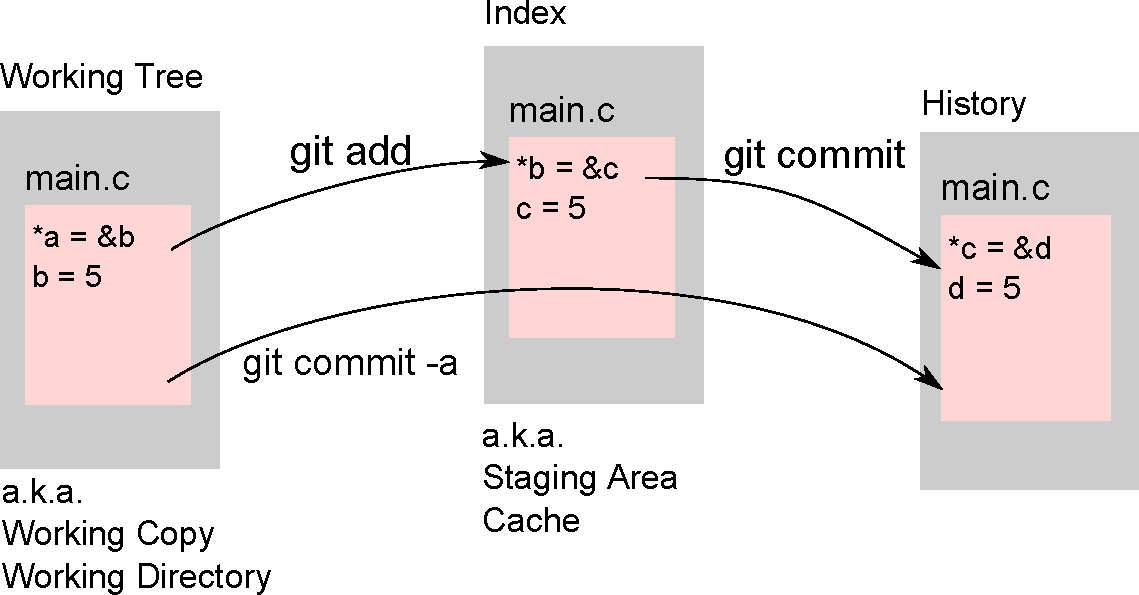
\includegraphics[height=50mm]{add_commit.pdf}
        \mode<article>{
          \caption{Relationship between the Working Tree, the Index
            and the History}
          \label{fig:stagecommit}
        }
      \end{center}
    \end{figure}

  }

  \only<3>{
    \begin{itemize}
    \item Tracked file - a file that is in the index
    \item Untracked file - any other file in the working copy
    \end{itemize}

    \begin{itemize}

    \item \texttt{git commit -a} updates all tracked files
    \item You can use .gitignore to ignore untracked files according to
      a list of wildcard patterns.

    \end{itemize}
  }

  \mode<article>{ The following code snippet illustrates the workflow
    for adding untracked files to the history, with explicit
    \texttt{add} and \texttt{commit} commands.
  }%

\defverbatim[colored]\screensession{%
\begin{lstlisting}
>> ls -ap
./ ../ .git/
>> vi main.c
>> git status
# On branch master
# Untracked files:
#     main.c
>> git add main.c
>> git status
# On branch master
# Changes to be committed:
#     new file:   main.c
>> git commit
>> git status
# On branch master
nothing to commit (working directory clean)
\end{lstlisting}
}


  \only<4>{
    Adding a new file
    \screensession
  }

  \mode<article>{ The following code snippet illustrates that even
    when a file is already tracked, you still need to perform an
    \texttt{add} command before trying to \texttt{commit} the new
    version.
  }%

\defverbatim[colored]\screensession{%
\begin{lstlisting}
>> vi main.c
>> git status
# On branch master
# Changed but not updated:
#     modified:   main.c
>> git add main.c
>> git status
# On branch master
# Changes to be committed:
#     modified:   main.c
>> git commit
>> git status
# On branch master
nothing to commit (working directory clean)
\end{lstlisting}
}

  \only<5>{
    Editing an existing file
    \screensession
  }


  \mode<article>{ And finally, the following snippet demonstrates how
    the \texttt{-a} switch for the \texttt{commit} command will
    automatically \texttt{add} the tracked files before committing.
  }%


\defverbatim[colored]\screensession{%
\begin{lstlisting}
>> vi main.c
>> git status
# On branch master
# Changed but not updated:
#     modified:   main.c
>> git commit -a
>> git status
# On branch master
nothing to commit (working directory clean)
\end{lstlisting}
}

  \only<6>{
    Editing an existing file (commit -a)
    \screensession
  }


\end{frame}

\subsection{Distributed Version Control}

Up to this point we have been telling you that Git is a decentralized
or distributed version control system, but we haven't given much
background on what that means.

The first thing to understand is that the history of a
Git repository is ``portable'', meaning that it is not attached to one
particular repository, as opposed, for instance, to how Subversion
uses a UUID in the repository and the revisions are attached to that
UUID.

In Git, the history does not carry any fundamental information that
attaches the data to one particular repository. The
history can be freely transferred from one place to another and the
different copies of that history can diverge and converge in time
without much regulation.

In a practical sense, this means every instance of the repository
contains the entire data set of the revision history, and
technically, is completely stand-alone to continue the development.

In order to diverge and converge different revisions in different
repositories, you use the \texttt{clone}, \texttt{fetch},
\texttt{push} and \texttt{pull} commands.

The most important concept to understand, however, is that there is no
such thing as ``the central repository''. As Figure
~\ref{fig:decentralized} illustrates, each repository is free to
exchange information with every other peer, and DevGit is a
canonical repository only as a convention adopted by the developers.

\begin{frame}[fragile]
  \frametitle{Distributed version control}

  \only<2>{
    \begin{itemize}
    \item Each developer has a full repository
    \item No central repository
    \item Canonical repository by convention
    \item All repositories are equal
    \item Peer-to-peer code sharing
    \end{itemize}

    \begin{figure}
      \begin{center}
        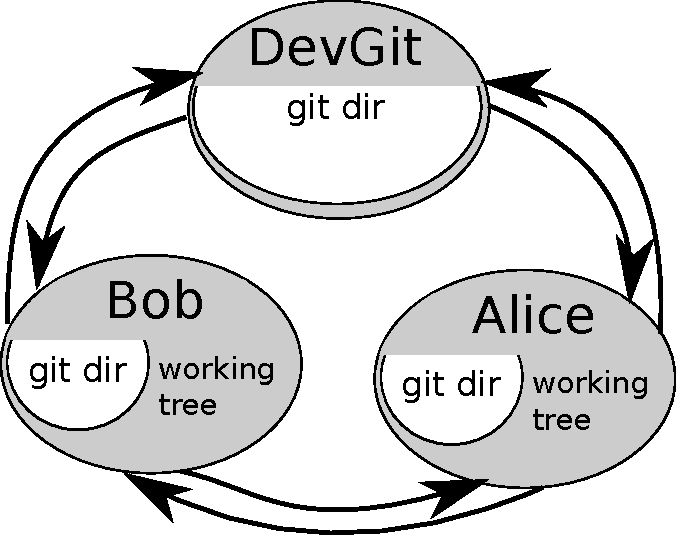
\includegraphics[height=30mm]{decentralized.pdf}
        \mode<article>{
          \caption{Relationship between Git repositories sharing the
            same history}
          \label{fig:decentralized}
        }
      \end{center}
    \end{figure}
  }

\defverbatim[colored]\screensession{%
\begin{lstlisting}
>> git clone devgit:mygroup/myrepo
>> cd myrepo
>> ls -ap
./ ../ .git/ main.c
>> git remote -v
origin devgit:mygroup/myrepo (fetch)
origin devgit:mygroup/myrepo (push)
\end{lstlisting}
}

  \only<3>{
    Cloning remembers where it came from
    \screensession
  }

\end{frame}

The \texttt{clone} command will initialize a new repository,
register the given URL as a remote repository by the nickname
\texttt{origin}, get a full copy of the entire history from that remote
repository and checkout the \texttt{master} branch to the working
tree.

The \texttt{remote -v} command here is used just to illustrate that
the relationship with the \texttt{origin} repository is completely
configurable. You can add additional remote repositories and
synchronize with those as well.

We are going to cover the \texttt{fetch}, \texttt{pull} and
\texttt{push} commands later. 

\subsection{Non-linear history}

The Git repositories start out sharing the same history, but will
diverge as changes are committed.  There needs to be a way for them
to converge to get back in sync.

Instead of trying to serialize the changes to get them into some
canonical order, Git adopts the strategy of representing the
history as a Directed Acyclic Graph of commits.  It is directed
because each link points from a commit to its parent, where the
parent is the commit that it derives from (its previous version).
A merge results in a commit having more than one parent.  This
means that the combined history will actually represent the way the
history diverged and reconverged in the independent repositories.

Also, a commit in Git does not represent a delta (set of source
changes) as in traditional systems.  It represents a snapshot of
the state of the source code at a point in time.  You can think of
this as a tar or zip file of the source code stored in each node of
the Directed Acyclic Graph (this is not how it is actually
implemented -- it is far more efficient).  This may seem like a
trivial difference, but you will come to realize just how
fundamental this difference is to the way Git represents history
and in turn how branching works.

This is a very significant change from other revision control systems,
especially the ones that are centralized. Figure ~\ref{fig:linear}
illustrates the difference in the scenarios of linear history versus
non-linear history when users make concurrent changes to
files.


\begin{frame}[fragile]
  \frametitle{Non-linear history}

  \only<2-4>{%
    \mode<article>{
      \setcounter{subfigure}{0}
    }%
    \begin{figure}[p]%
      \begin{center}%
        \only<2>{%
          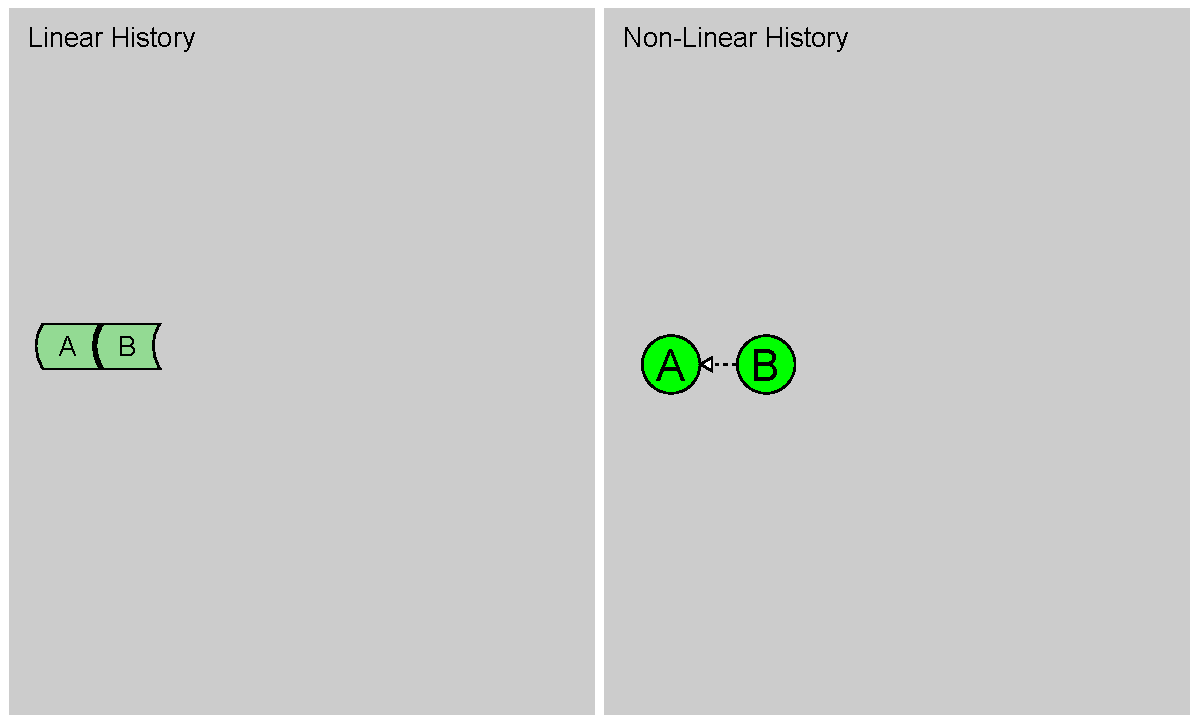
\includegraphics[height=50mm]{linear_history_1.pdf}%
          \mode<article>{
            \subcaption{Initial state of the history}
            \label{fig:linear:initial}
          }%
        }%
        \only<3>{%
          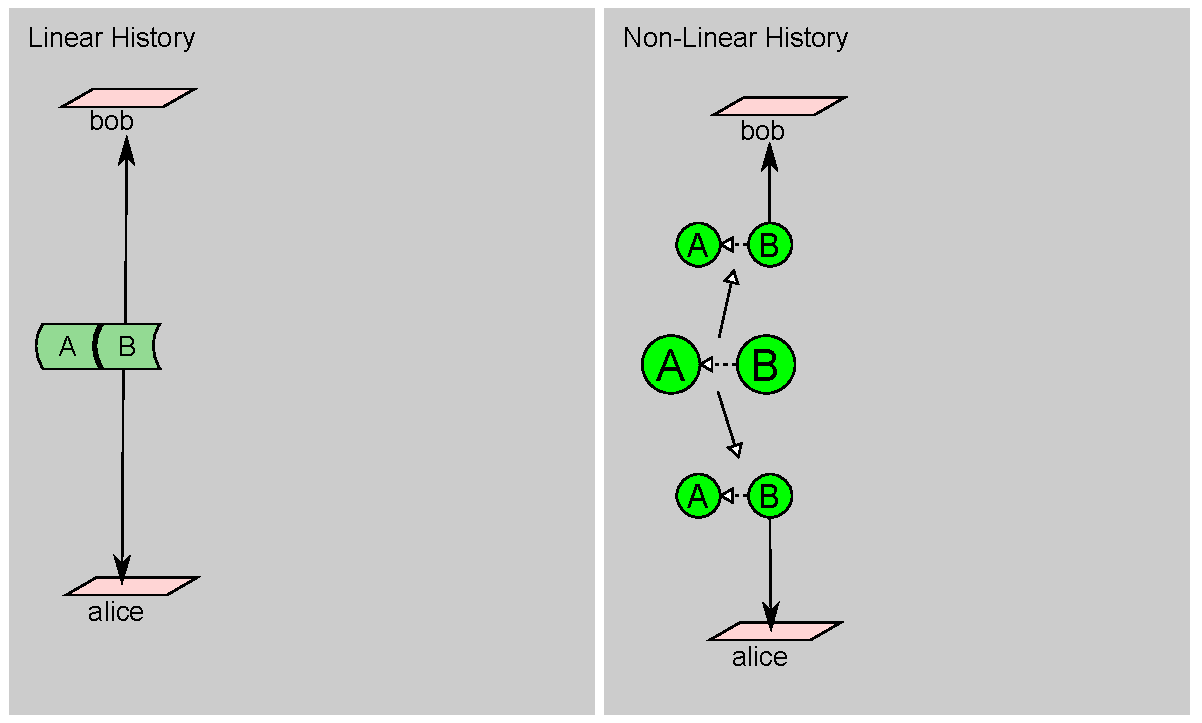
\includegraphics[height=50mm]{linear_history_2.pdf}%
          \mode<article>{
            \subcaption{Alice and Bob get their working copies}
            \label{fig:linear:clone}
          }%
        }%
        \only<4>{%
          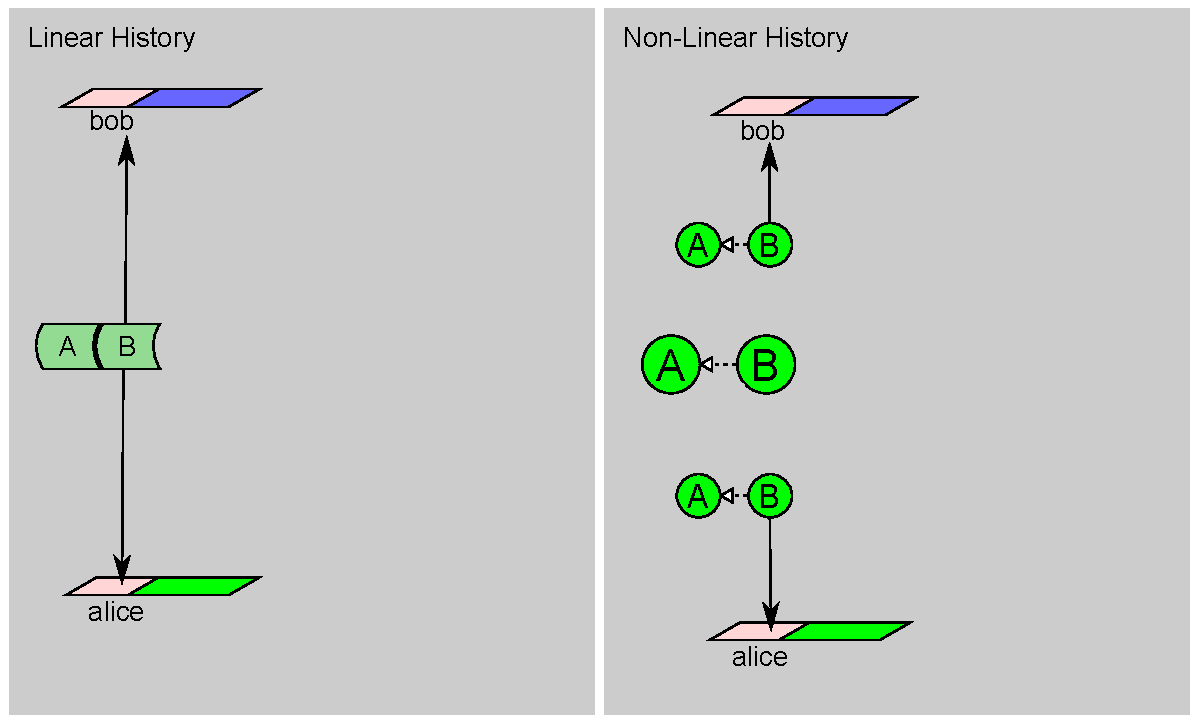
\includegraphics[height=50mm]{linear_history_3.pdf}%
          \mode<article>{
            \subcaption{Alice and Bob make local changes}
            \label{fig:linear:changes}
          }%
        }%
      \end{center}%
      \mode<article>{
        \begin{center}
          Fig ~\ref{fig:linear} continues on next page
        \end{center}
      }%
    \end{figure}%
  }%
  \only<5-7>{%
    \mode<article>{
      \setcounter{subfigure}{3}
    }%
    \begin{figure}[p]%
      \begin{center}%
        \only<5>{%
          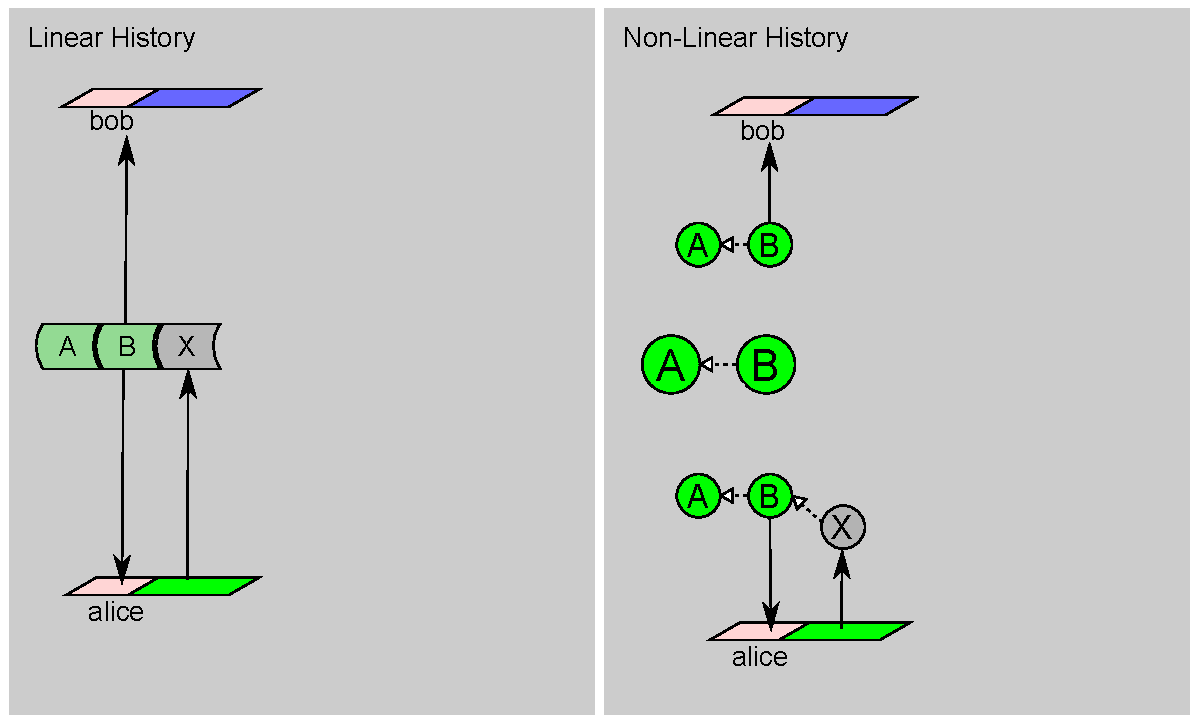
\includegraphics[height=50mm]{linear_history_4.pdf}%
          \mode<article>{
            \subcaption{Alice commits her changes}
            \label{fig:linear:alicecommit}
          }%
        }%
        \only<6>{%
          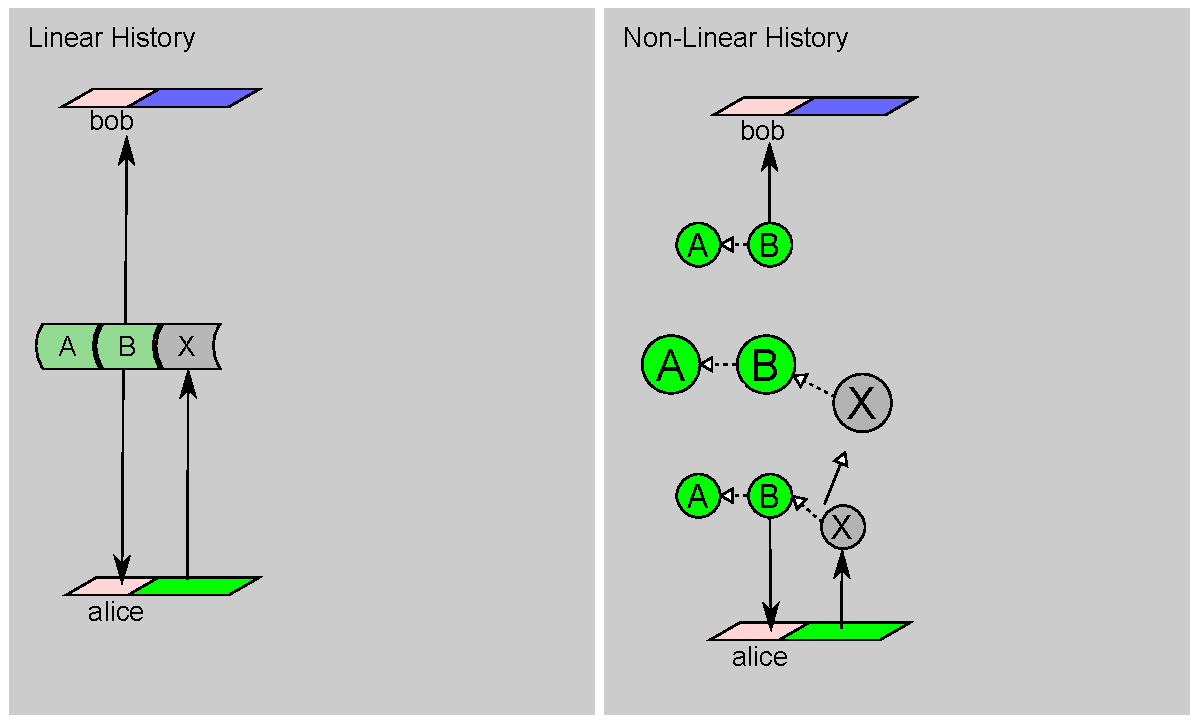
\includegraphics[height=50mm]{linear_history_5.pdf}%
          \mode<article>{
            \subcaption{Since the commit in Git is local, Alice needs to push it}
            \label{fig:linear:alicepush}
          }%
        }%
        \only<7>{%
          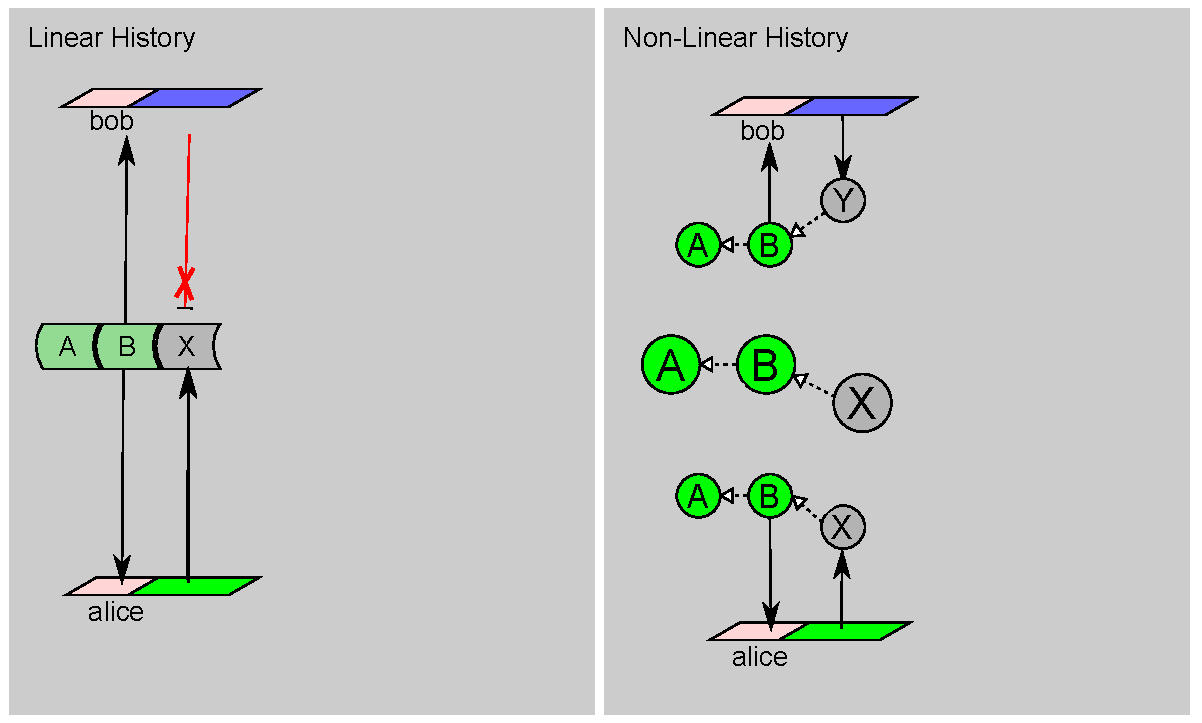
\includegraphics[height=50mm]{linear_history_6.pdf}%
          \mode<article>{ \subcaption{Now, Bob tries to commit and fails
              on the linear history scenario, while succeeds in the
              non-linear scenario}
            \label{fig:linear:bobcommit}
          }%
        }%
      \end{center}%
      \mode<article>{
        \begin{center}
          Fig ~\ref{fig:linear} continues on next page
        \end{center}
      }%
    \end{figure}%
  }%
  \only<8-10>{%
    \mode<article>{
      \setcounter{subfigure}{6}
    }%
    \begin{figure}[p]%
      \begin{center}%
        \only<8>{%
          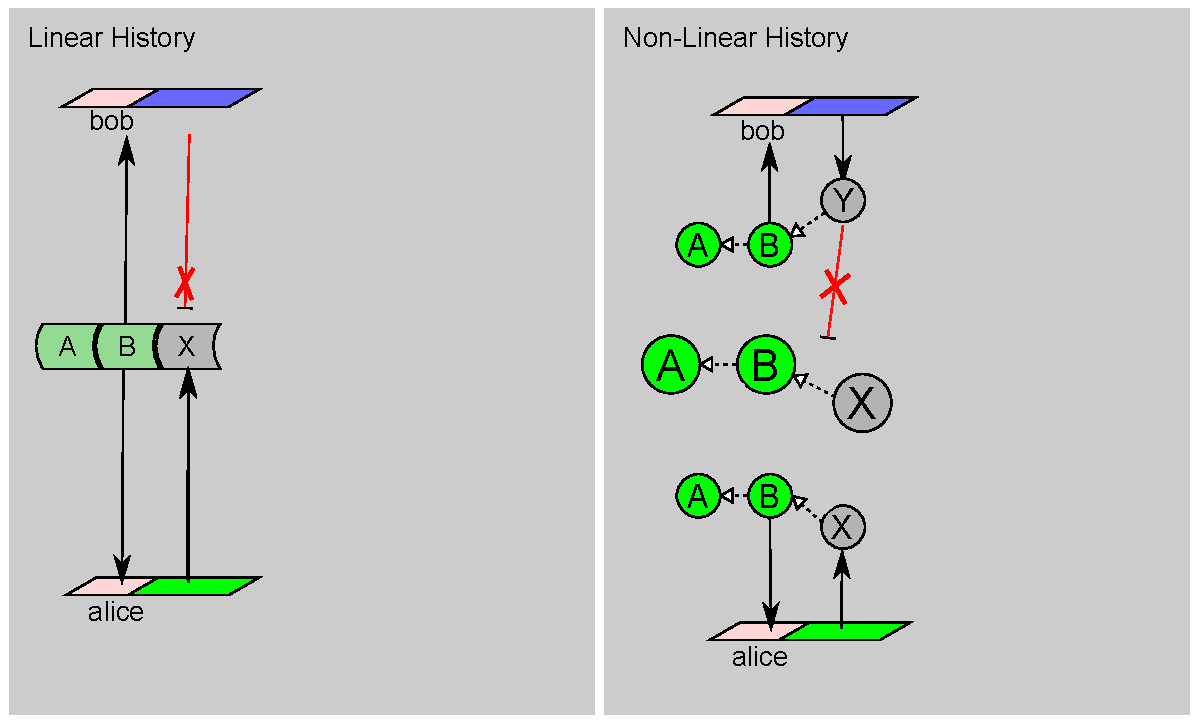
\includegraphics[height=50mm]{linear_history_7.pdf}%
          \mode<article>{ \subcaption{But Bob can't push, because he
              doesn't have the most up-to-date version}
            \label{fig:linear:bobpushfail}
          }%
        }%
        \only<9>{%
          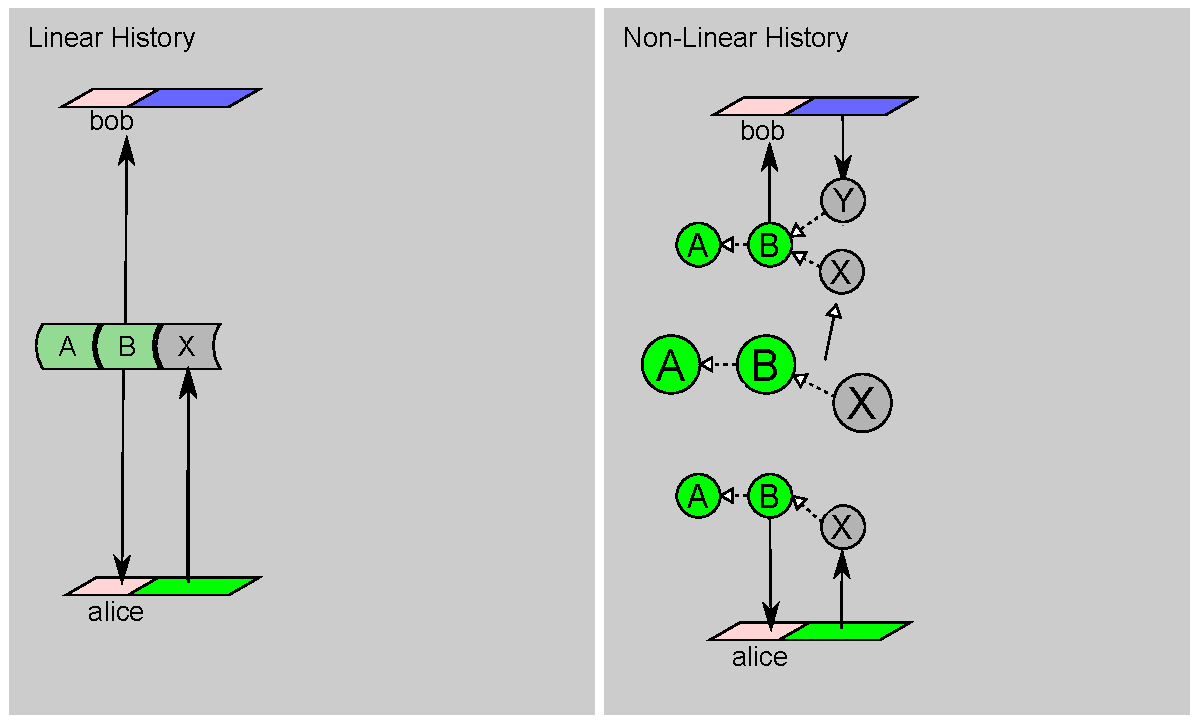
\includegraphics[height=50mm]{linear_history_8.pdf}%
          \mode<article>{
            \subcaption{Bob fetches the new changes submitted by Alice}
            \label{fig:linear:bobfetch}
          }%
        }%
        \only<10>{%
          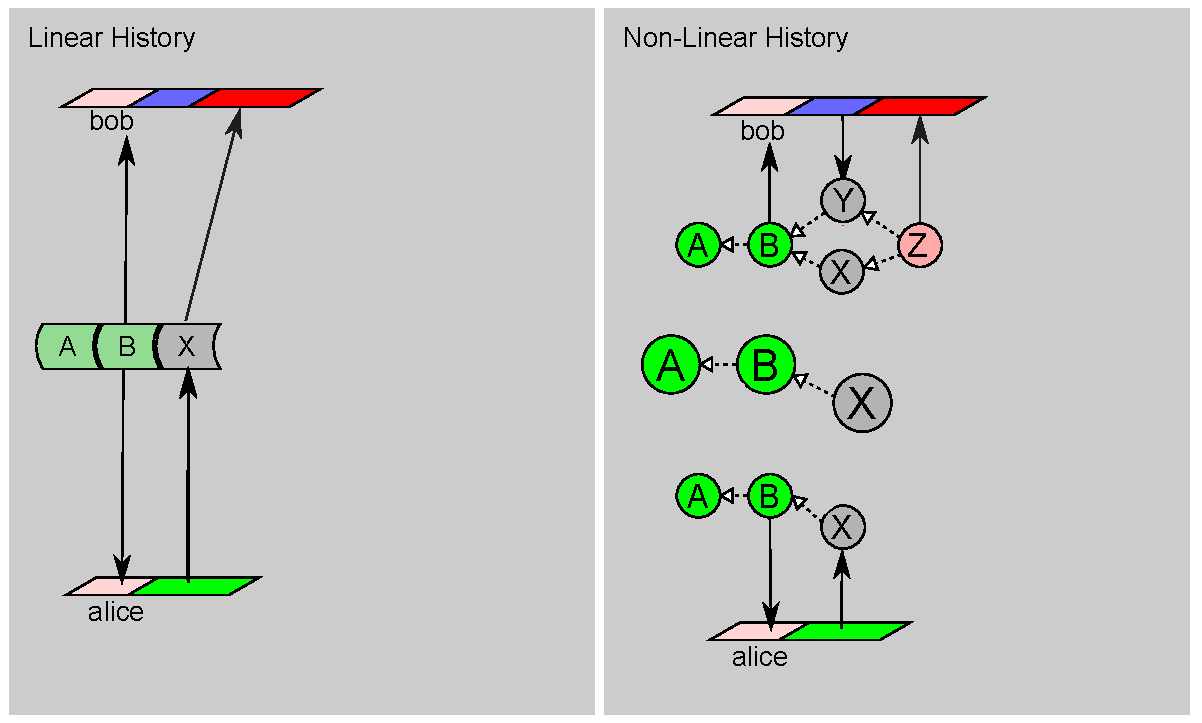
\includegraphics[height=50mm]{linear_history_9.pdf}%
          \mode<article>{
            \subcaption{Bob merges the changes into his working
	    copy, note that the merge has two parent nodes}
            \label{fig:linear:bobmerges}
          }%
        }%
      \end{center}%
      \mode<article>{
        \begin{center}
          Fig ~\ref{fig:linear} continues on next page
        \end{center}
      }%
    \end{figure}%
  }%
  \only<11-13>{%
    \mode<article>{
      \setcounter{subfigure}{9}
    }%
    \begin{figure}[p]%
      \begin{center}%
        \only<11>{%
          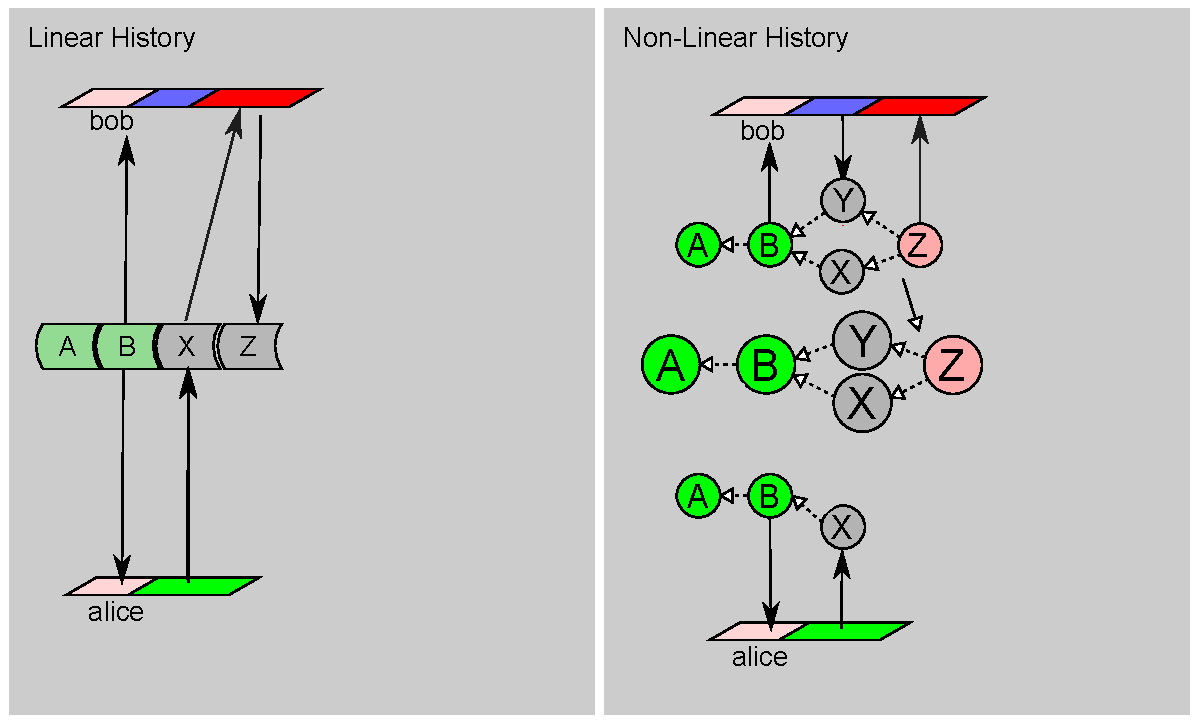
\includegraphics[height=50mm]{linear_history_10.pdf}%
          \mode<article>{
            \subcaption{Now, Bob succeeds in sending the new version to the server}
            \label{fig:linear:bobpush}
          }%
        }%
        \only<12>{%
          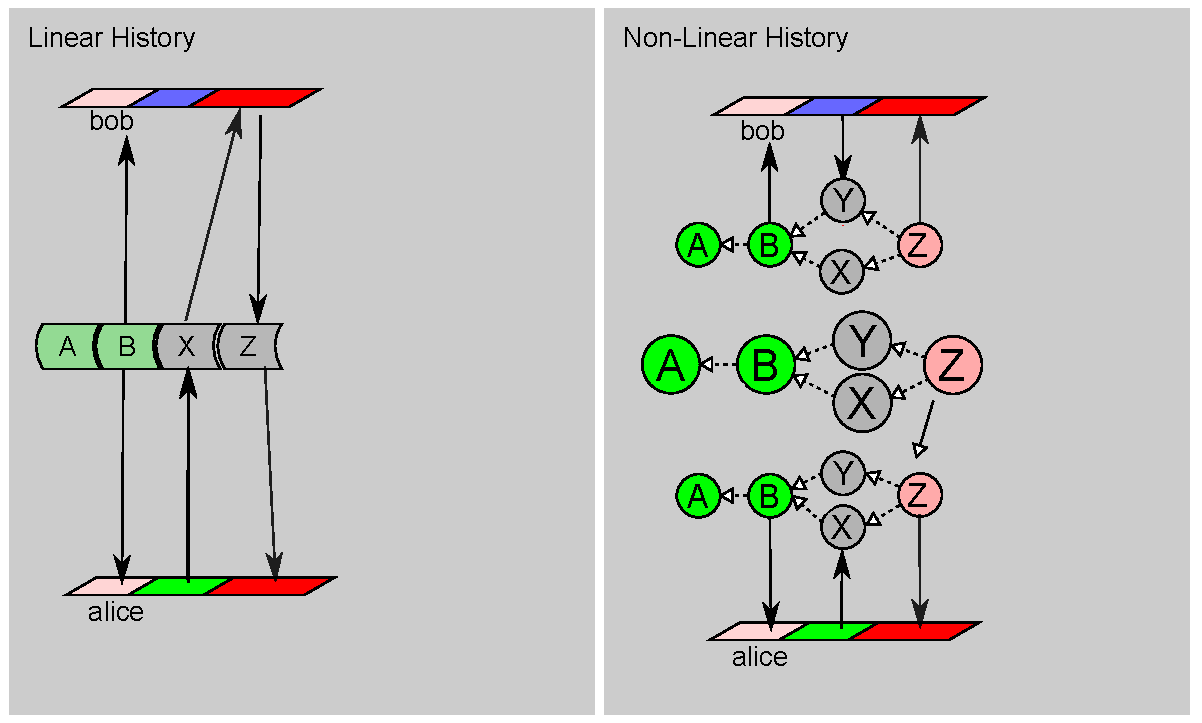
\includegraphics[height=50mm]{linear_history_11.pdf}%
          \mode<article>{
            \subcaption{And Alice can get the changes submitted by Bob}
            \label{fig:linear:alicepull}
          }%
        }%
        \only<13>{%
          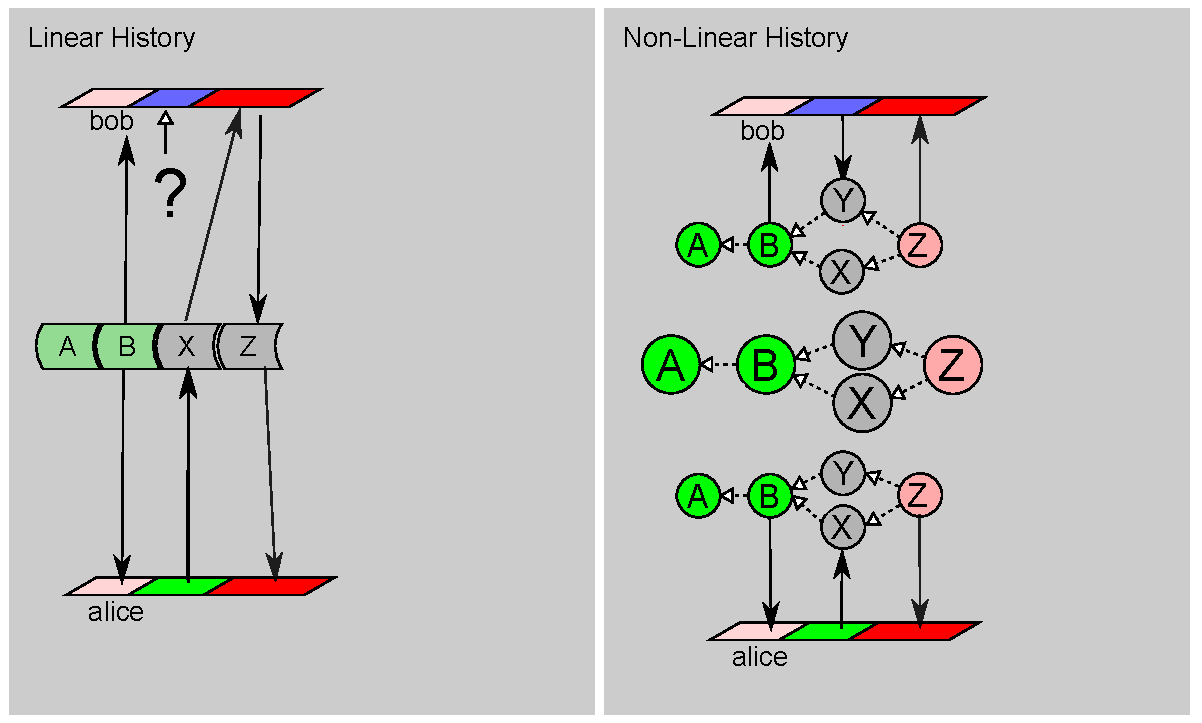
\includegraphics[height=50mm]{linear_history_12.pdf}%
          \mode<article>{ \subcaption{Final state of the history, but
              the initial changes made by Bob were lost in the linear
              scenario because it has not way to represent it}
            \label{fig:linear:final}
          }%
        }%
      \end{center}%
      \mode<article>{
        \caption{Comparison of linear and non-linear history}
        \label{fig:linear}
      }%
    \end{figure}%
  }%

  \only<14>{
    \begin{itemize}
    \item Each commit is a ``snapshot'', not a diff
    \item Commits form a directed acyclic graph
    \item Connected by parent pointers
    \item Numbering revisions just causes confusion
    \item Git does not use serial revision numbers
    \item Git uses SHA1 checksum instead
    \end{itemize}
  }

\end{frame}

The way Git identify the revisions is also something that is
surprising for most people with experience in other version control
systems, since there isn't a serial numbering of the revisions.
If you think about it for a second you will realize that since Git
has a non-linear history, it's very hard to
define, looking at Figure ~\ref{fig:linear:bobcommit}, which one would
receive the next serial number.

What Git uses instead is a SHA1 checksum of the commit data (which
includes the parent commit's SHA1, the date, the author and the message)
to identify the commit. And this ID is unique and immutable in the
history of the repository\footnote{This is how Git implements the
  cryptographic authentication of its history. Basically, the commit
  ID recursively includes the checksum of all previous versions of
  the source code.  You can see more information on that subject on
  \url{http://www.kernel.org/pub/software/scm/git/docs/user-manual.html\#trust}.}.

\subsection{Pull-push workflow}

In this section we cover the process used to synchronize one
repository -- the ``local'' -- to one or more external repositories --
the ``remotes''. It's important to understand this terminology, since
you'll be dealing with it a lot.

\begin{enumerate}
\item[Local]{This term refers to the Git repository you are
  working in. Since there is no technical difference between the
  repositories, this is just a matter of perspective. The local is
  where you are.}
\item[Remote]{This term refers to any other repository you might
  interact with. It includes, but is not limited to,
  the repository from which you cloned. You can have any number of
  remotes configured.}
\end{enumerate}

\begin{frame}[fragile]
  \frametitle{Pull-push workflow}

  \only<2>{
    \begin{itemize}
    \item Commit stores a snapshot in \underline{local} repo
    \item Use a canonical repo (on DevGit) to share
    \item Use peer-to-peer to share
    \end{itemize}
  }
  \only<3>{
    \begin{itemize}
    \item \texttt{git push} - send local changes to remote repo
    \item \texttt{git fetch} - get changes from remote repo
    \item \texttt{git pull} - runs fetch then runs merge to \underline{current} branch
      \begin{itemize}
      \item Use fetch, not pull when you don't want the merge
      \end{itemize}
    \end{itemize}
  }

  \only<4->{%
    \mode<article>{
      \setcounter{subfigure}{0}
    }%
    \begin{figure}[p]%
      \begin{center}%
        \only<4>{%
          \begin{minipage}[t]{0.4\linewidth}
            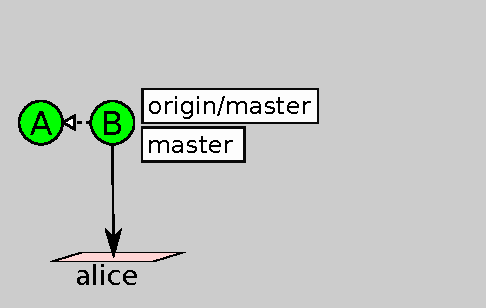
\includegraphics[height=30mm]{pull_push_2.pdf}%
            \mode<article>{
              \subcaption{Initial state, both remote and local ``master'' point to the same commit}
              \label{fig:pushpull:initial}
            }%
          \end{minipage}
        }%
        \only<5>{%
          \begin{minipage}[t]{0.4\linewidth}
            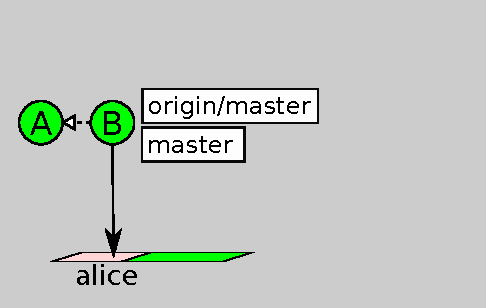
\includegraphics[height=30mm]{pull_push_3.pdf}%
            \mode<article>{
              \subcaption{Local changes are made in the working copy}
              \label{fig:pushpull:change}
            }%
          \end{minipage}
        }%
        \only<6>{%
          \begin{minipage}[t]{0.4\linewidth}
            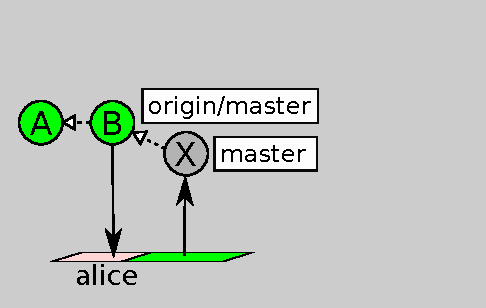
\includegraphics[height=30mm]{pull_push_4.pdf}%
            \mode<article>{
              \subcaption{A local commit moves the local ``master'' reference}
              \label{fig:pushpull::commit}
            }%
          \end{minipage}
        }%
        \only<7>{%
          \begin{minipage}[t]{0.4\linewidth}
            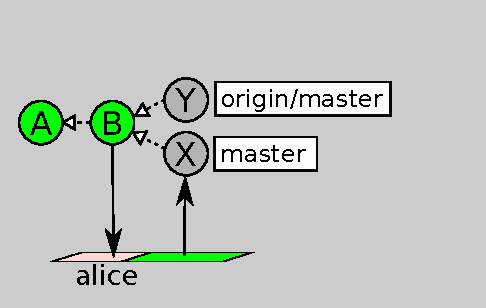
\includegraphics[height=30mm]{pull_push_5.pdf}%
            \mode<article>{
              \subcaption{The fetch operation updates the remote ``master'', which contains one new commit}
              \label{fig:pushpull:fetch}
            }%
          \end{minipage}
        }%
        \only<8>{%
          \begin{minipage}[t]{0.4\linewidth}
            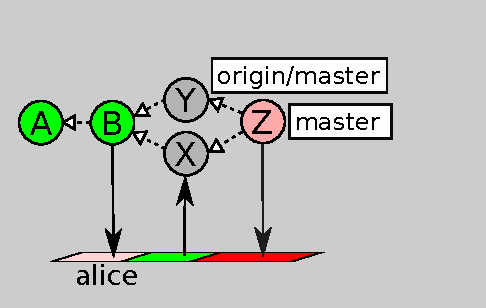
\includegraphics[height=30mm]{pull_push_6.pdf}%
            \mode<article>{
              \subcaption{The merge operation is used and generates a new commit, moving the local ``master''}
              \label{fig:pushpull:merge}
            }%
          \end{minipage}
        }%
        \only<9>{%
          \begin{minipage}[t]{0.4\linewidth}
            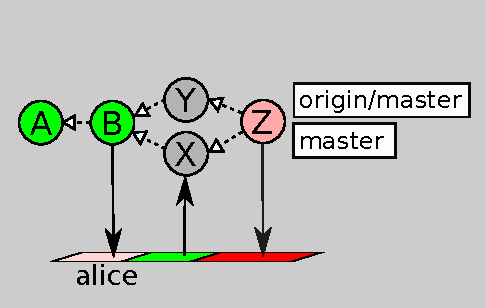
\includegraphics[height=30mm]{pull_push_7.pdf}%
            \mode<article>{
              \subcaption{The push operation updates the remote ``master'', since it's a fast-forward merge}
              \label{fig:pushpull:push}
            }%
          \end{minipage}
        }%
      \end{center}%
      \mode<article>{ \caption{Interactions between local and remote repository}
        \label{fig:pushpull}
      }%
    \end{figure}%
  }%
\end{frame}

By this point it should be clear that the \texttt{commit} operation
operates entirely in the local repository, and performs no action
outside that repository directory whatsoever. Therefore, in order to
share your recent commits with other developers you can either use a
canonical repository (e.g., on DevGit), or you can push and pull
directly to/from your peers\footnote{We are not going to cover the
  details on how to implement the peer-to-peer sharing workflow, but
  you can find more information at
  \url{http://progit.org/book/ch5-1.html}.}.

In a very strict sense, you need to understand that when two
developers (let's call them Alice and Bob) have copies of the same
branch (let's assume \texttt{master}), they actually have two
branches. The process of synchronizing changes between Alice's and
Bob's version of \texttt{master} is technically achieved by a
\texttt{merge} operation. The same operation you use when dealing with
different branches in your local repository. Figure
~\ref{fig:pushpull} illustrates what happens when the two developers
diverge and how they converge on their versions of the \texttt{master}
branch.


\subsection{Branching}

Branches in Git are also very different from other version control
systems.  As we saw in looking at non-linear history, commits
naturally form branch-like structures in the normal course of
multiple developers working on the ``main line'' (in Git this branch
is called master).

In Git, a Branch is just a pointer to some commit in the history (a
node in the directed acyclic graph).
These pointers are called references or refs for short.
In traditional systems, a branch is a sequence of versions and these
versions are an intergal part of the branch.
This is not true in Git.
We sometimes think of Git commits being on a branch, but it is more
correct to say that these commits are \emph{reachable} from the
branch, meaning that following the links, there is a path from the
ref to the given nodes (commits).
However, they may be reachable from several branches.
In Git, commits do not ``live'' on a branch.
It is important that you think of Git branches as pointers (refs),
not collections of commits, because it is quite common to add,
delete and move refs and therefore redefine what commits are ``on''
a branch (reachable from it).

In a more broad sense, a branch is one particular type of reference
that provides the feature that whenever you create a new commit in a
branch, the reference will be moved to the new commit. But, unlike
most revision control systems, there is no metadata stored in the
commit that identifies the branch where the commit was created.

This is just another consequence on how Git handles its history in a
non-linear way. Figure ~\ref{fig:linearbranching} illustrates the
difference between branches with linear and non-linear history. Note
that the two sides actually represent the same set of operations in a
given time-frame, but on the left side you clearly see which commits
where made in which branch, while on the right side, you can only see
that they have ``common ancestors''.

It's important to understand this concept, because once the branches merge
themselves back and forth -- as illustrated in Figure
~\ref{fig:linearbranching2} -- you can no longer tell for sure which
of the diverted paths were made in which branch. The only thing you
know is that all the commits are ``reachable'' from both branches.

When you read the Git documentation for the \texttt{log} and
\texttt{diff} commands, most ``revision ranges'' will be explained in
terms of graph operations, e.g., commit A is reachable from commit B
and from commit C.

\begin{frame}[fragile]
  \frametitle{Branching}

  \only<2>{
    \begin{itemize}
    \item A branch is a pointer (reference or ref) to a commit
    \item Commits don't ``live'' on a branch
    \item Some commits are reachable from a branch
    \end{itemize}
    \begin{figure}
      \begin{center}
        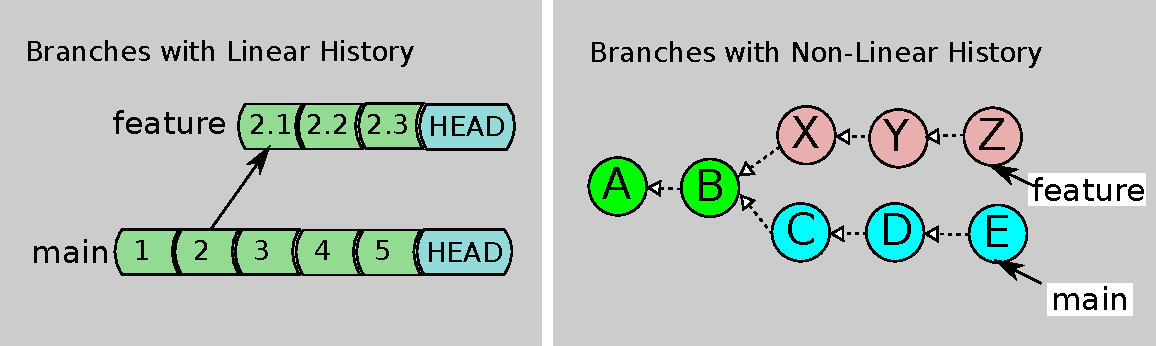
\includegraphics[height=30mm]{linear_branching.pdf}
        \mode<article>{ \caption{Difference between branches with
            linear history and non-linear history}
          \label{fig:linearbranching}
        }%
      \end{center}
    \end{figure}
  }

  \only<3>{
    \begin{itemize}
    \item The branches can be merged back and forth
    \item History is preserved, but not at which branch
    \end{itemize}
    \begin{figure}
      \begin{center}
        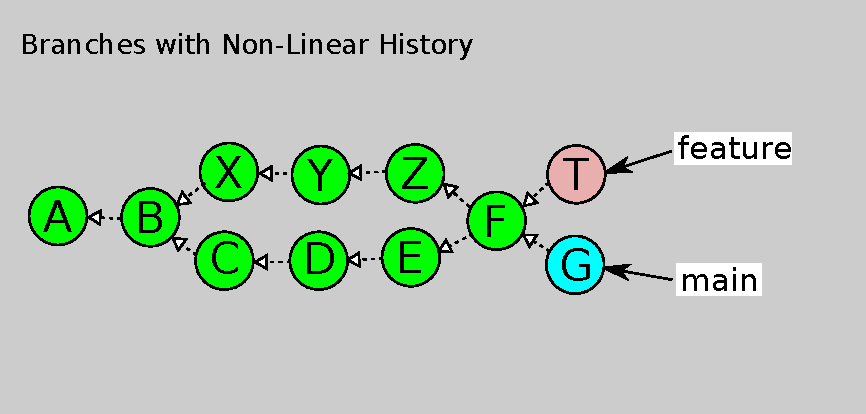
\includegraphics[height=30mm]{linear_branching_continued.pdf}
        \mode<article>{ \caption{Commits are ``reachable'' by any
            number of branches}
          \label{fig:linearbranching2}
        }%
      \end{center}
    \end{figure}
  }

  \mode<article>{

    One additional aspect you need to understand is the meaning of
    ``local branch'' and ``remote tracking branch''.

    \begin{enumerate}
      \item[Local Branch]{A ``normal'' branch in your local
        repository where you commit work.
        Its full name \emph{always} start with \texttt{refs/heads/}.}
      \item[Remote Tracking Branch]{A type of branch that tracks
        the location of a branch in another repository.
	This is not a true branch because the \texttt{commit}
	command will not move it as it does local branches.
	It is instead moved only when push and fetch detect that
	the branch in the remote repository has moved.
        They usually have their full name starting with
	\texttt{refs/remotes/} followed by the nickname of the
	remote repository (e.g., origin) and the name of the branch
	in the remote repository that it tracks.}
    \end{enumerate}

  }

  \only<4>{
    \begin{itemize}
    \item Local branches (moved by git commit)
      \begin{itemize}
      \item master (refs/heads/master)
      \item new\_feature (refs/heads/new\_feature)
      \end{itemize}
    \item Remote tracking branches (moved by git fetch and push)
      \begin{itemize}
      \item origin/master (refs/remotes/origin/master)
      \item origin/new\_feature (refs/remotes/origin/new\_feature)
      \item origin/bugfix (refs/remotes/origin/bugfix)
      \item These are not true branches, just references
      \end{itemize}
    \end{itemize}
  }

  \mode<article>{

    We now follow to some commands that exemplify how to work with
    branches in Git.

    In the first snippet, we use the \texttt{branch -a} command to
    list all local and remote tracking branches. Then we create a
    new local branch, \texttt{bugfix}, from the
    \texttt{origin/bugfix} remote tracking branch by using the
    \texttt{checkout -t} command. The tracking information is used by
    the \texttt{status} and \texttt{pull} commands. We then repeat the
    \texttt{branch -a} command to show that not only a new branch was
    created but we actually switched to that branch (the \texttt{*}
    is now in front of it).

  }

\defverbatim[colored]\screensession{%
\begin{lstlisting}
>> git branch -a
* master
  remotes/origin/master
  remotes/origin/bugfix
>> git checkout -t origin/bugfix
>> git branch -a
  master
* bugfix
  remotes/origin/master
  remotes/origin/bugfix
\end{lstlisting}
}

  \only<5>{
    Getting a remote branch
    \screensession
  }

  \mode<article>{

    In this second snippet, we use the \texttt{-b} option instead of
    the \texttt{-t}, because we don't want to setup tracking
    information between \texttt{mynewfeature} and
    \texttt{origin/master}.  \texttt{origin/master} is just the
    starting point of the new branch.
    We later use the \texttt{push -u}
    command which will create the \texttt{mynewfeature} branch in the
    \texttt{origin} remote repository and set the tracking information
    for the \texttt{origin/mynewfeature} tracking branch instead.

  }

\defverbatim[colored]\screensession{%
\begin{lstlisting}
>> git checkout -b mynewfeature origin/master
>> git branch -a
  master
* mynewfeature
  bugfix
  remotes/origin/master
  remotes/origin/bugfix
>> git push -u origin mynewfeature
>> git branch -a
  master
* mynewfeature
  bugfix
  remotes/origin/master
  remotes/origin/mynewfeature
  remotes/origin/bugfix
\end{lstlisting}
}

  \only<6>{
    Creating a new branch
    \screensession
  }

\end{frame}

Traditional version control systems implement the concept of
branches in terms of a set of names in a ``global namespace''.
Implementations differ from one system to another, but as the
version control takes place in a centralized location, branch names
are global and visible to all developers.

Git is a decentralized version control system, having no concept of a global
namespace. Each repository -- be it on a server or in a developer's home
directory -- contains its own namespace. In general, therefore, developers
agree to a canonical repository in which to share code. But this canonical
repository is not different from any other repository as far as the Git
software is concerned; like every other repository, it contains its own
namespace.  A group's DevGit repository serves as the canonical repository for
that group.

The canonical repository does not need to list
all the branches in all the repositories. Users are free to decide
which branches they ``fetch'' from other repositories and which branches
they push to other repositories. Git calls branches fetched from other
repositories ``remote tracking branches''.

Note that it is \emph{technically} possible to fetch refs from completely
unrelated Git repositories into a single repository and even do merge
operations between them. What makes it possible is the fact that a ref is
simply a pointer to a node in a directed acyclic graph (DAG). When you fetch a
ref, you fetch the referenced node and, recursively, all nodes referenced by
it.

The ``pull'' command will, in addition to running the ``fetch''
command, perform a merge operation on the associated remote ref onto
the \emph{current} branch.

A ``push'', on the other hand, is the process by which you send, from
your repository (the local) to another repository (the remote)
a request to update a ref in the remote repository
to reference a particular node, while sending, recursively, the node and all
nodes referenced by it.

In order to ensure consistency across repositories, Git defines the concept of
``fast forward merge''. A fast forward merge happens when you are updating a
ref to refer to node B instead of node A, and B has A as an
\emph{ancestor}. Git will not allow ``non-fast-forward'' pushes unless a force
switch is provided, because doing so would mean overwriting someone else's
work. Take a look at Fig. ~\ref{fig:merges} for diagrams of the different
types of merges.

In practical terms, what happens when you do a push is that you are sending a
set of commits from your (local) repository to another (remote) repository in a
single operation, while sending to the remote the entire development history
behind those commits. When other developers fetch from that repository, they
will get a copy of the entire history of your work.

In Git, the default name for the integration branch is \texttt{master}, in the
same sense that Subversion uses \texttt{trunk}. Each local clone of a remote
repository has its own \texttt{master} branch that needs to be synchronized
with the remote repository, usually via the ``pull'' command.

\begin{frame}[fragile]
  \frametitle{Branching}

  \only<1>{
    \begin{figure}
      \begin{center}
        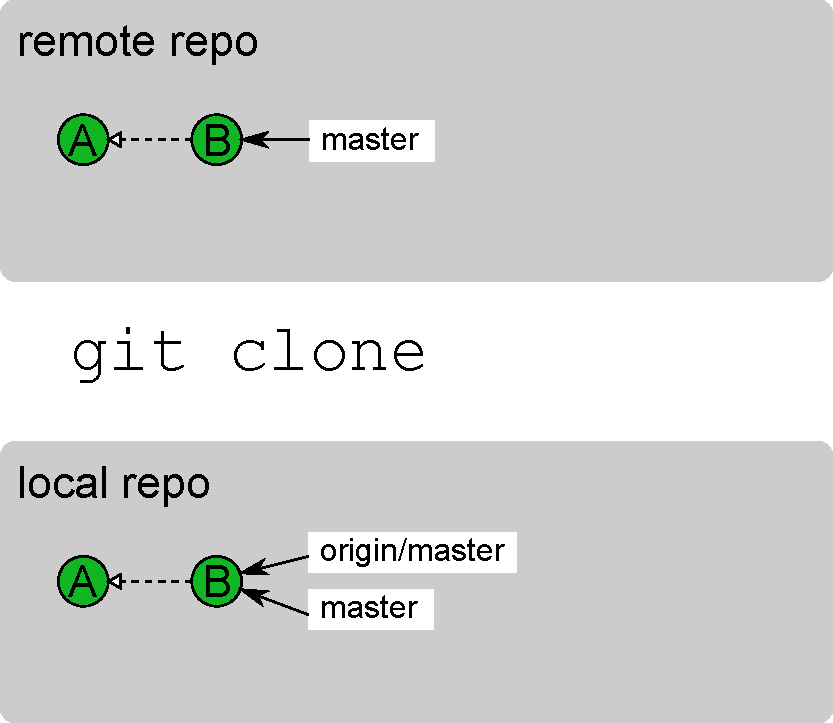
\includegraphics[height=50mm]{tracking_branches_1.pdf}
        \mode<article>{ \caption{Start by cloning a remote repository.}
        }%
      \end{center}
    \end{figure}
  }

  \only<2>{
    \begin{figure}
      \begin{center}
        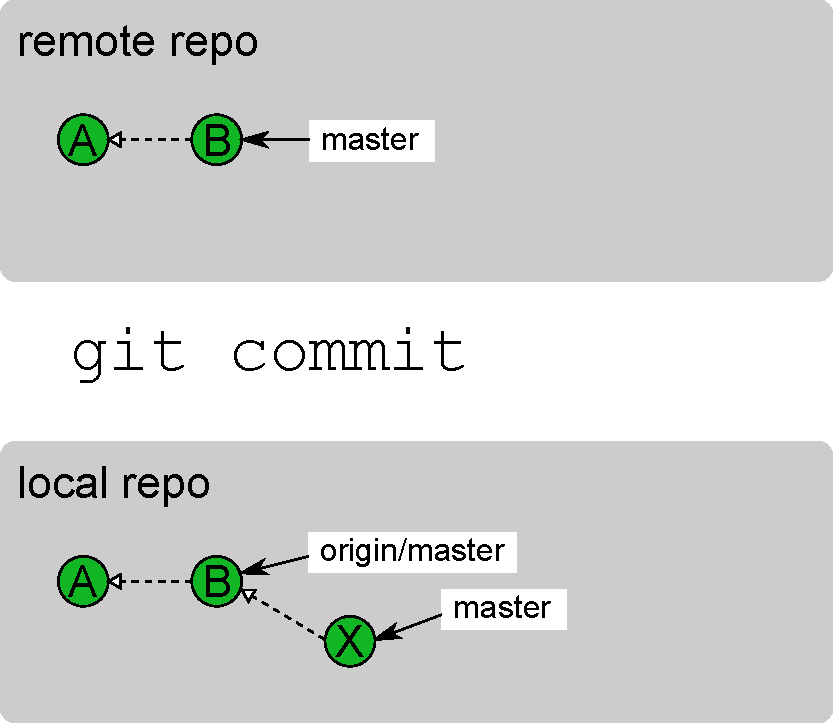
\includegraphics[height=50mm]{tracking_branches_2.pdf}
        \mode<article>{ \caption{Make some local changes (the commit
	does not affect the remote repository).}
        }%
      \end{center}
    \end{figure}
  }

  \only<3>{
    \begin{figure}
      \begin{center}
        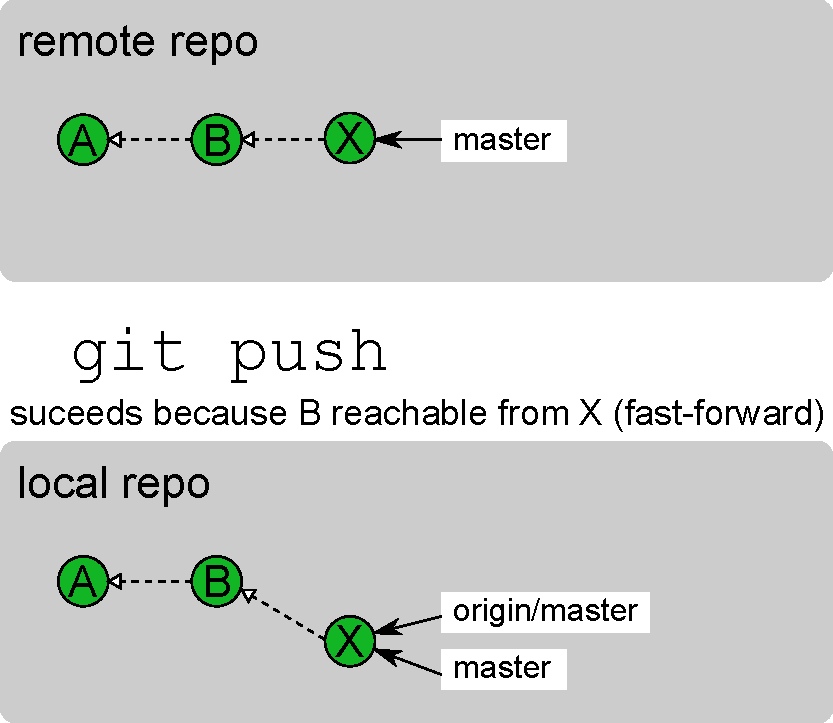
\includegraphics[height=50mm]{tracking_branches_3.pdf}
        \mode<article>{ \caption{Push the changes to the remote repository.
	This succeeds because the remote branch is reachable from the
	local branch.}
        }%
      \end{center}
    \end{figure}
  }

  \only<4>{
    \begin{figure}
      \begin{center}
        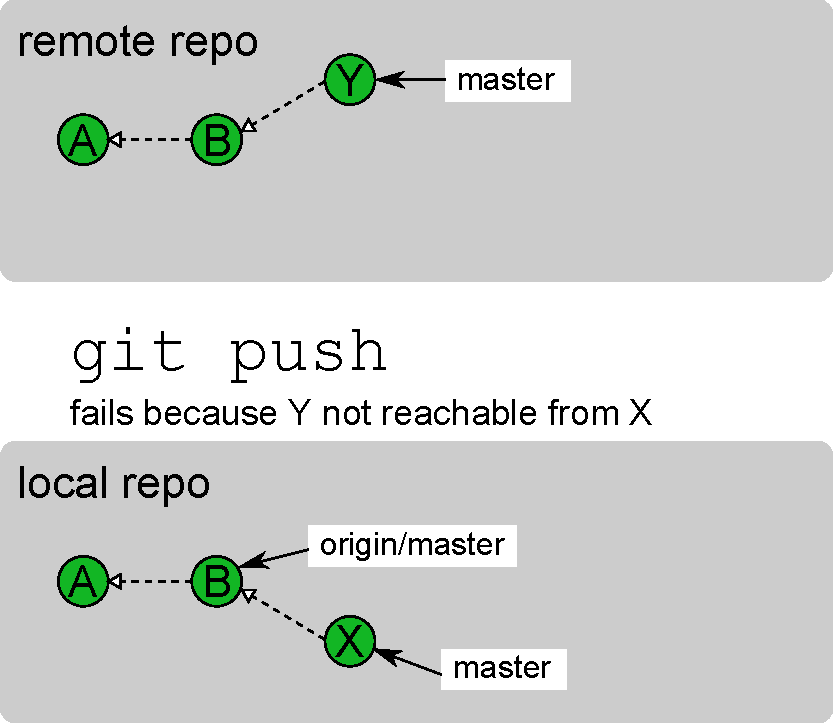
\includegraphics[height=50mm]{tracking_branches_4.pdf}
        \mode<article>{ \caption{But, what if someone else had pushed
	before you? In this case the remote branch is not reachable
	from the local branch.}
        }%
      \end{center}
    \end{figure}
  }

  \only<5>{
    \begin{figure}
      \begin{center}
        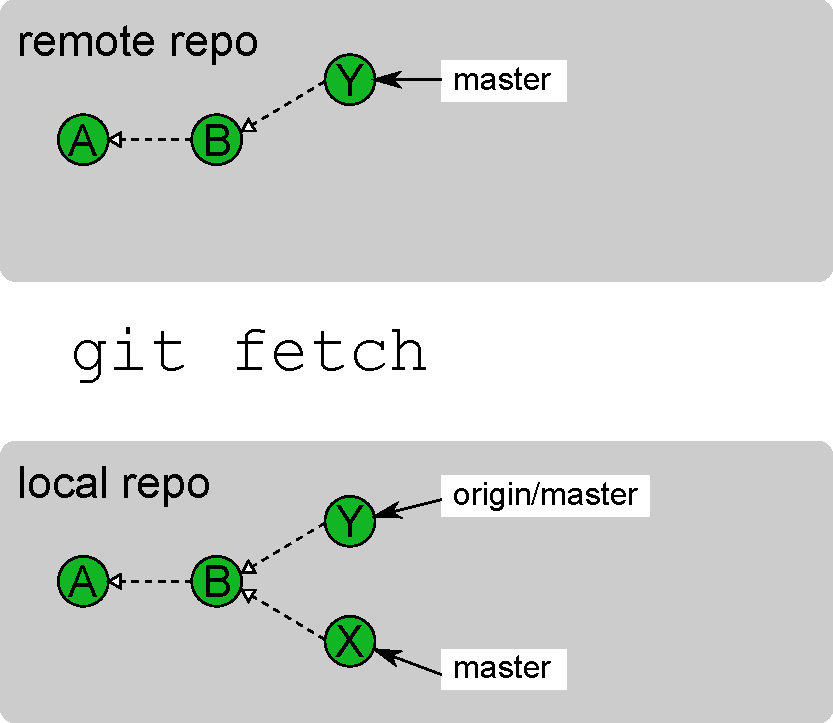
\includegraphics[height=50mm]{tracking_branches_5.pdf}
        \mode<article>{ \caption{So, fetch the remote changes into
	the local repository.}
        }%
      \end{center}
    \end{figure}
  }

  \only<6>{
    \begin{figure}
      \begin{center}
        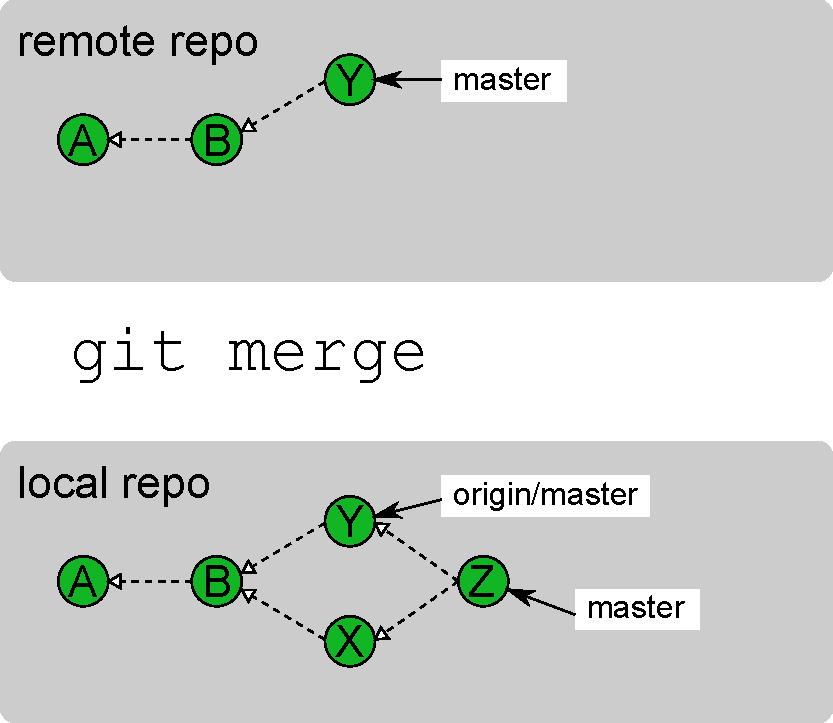
\includegraphics[height=50mm]{tracking_branches_6.pdf}
        \mode<article>{ \caption{Then, merge your work with their's.
	Note, pull would have performed the fetch and merge in
	one step.}
        }%
      \end{center}
    \end{figure}
  }

  \only<7>{
    \begin{figure}
      \begin{center}
        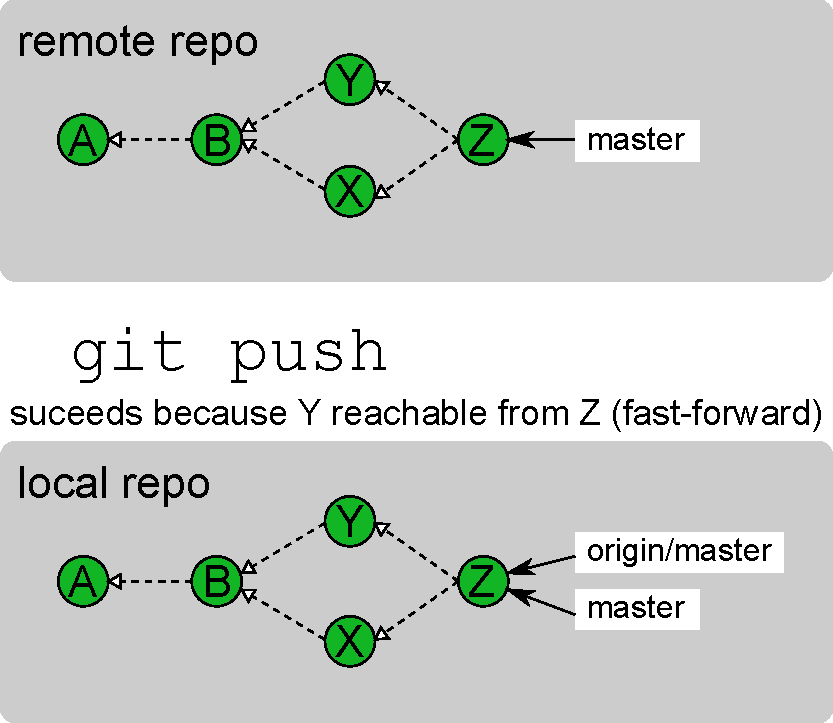
\includegraphics[height=50mm]{tracking_branches_7.pdf}
        \mode<article>{ \caption{Now, you can push the merged version.
	It will succeed because the remote branch is now reachable
	from the local branch.}
        }%
      \end{center}
    \end{figure}
  }

  \only<8>{
    \begin{figure}
      \begin{center}
        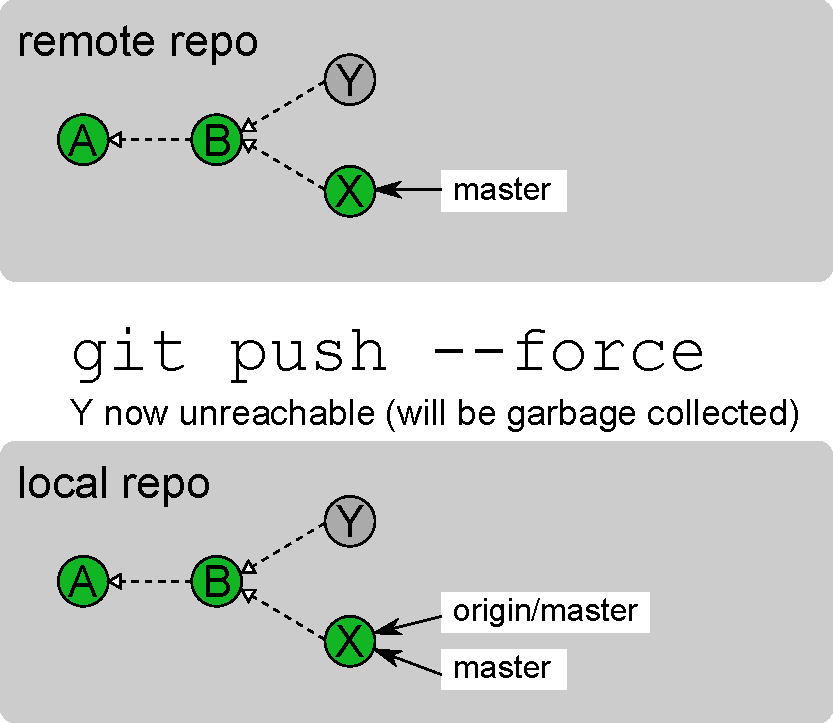
\includegraphics[height=50mm]{tracking_branches_8.pdf}
        \mode<article>{ \caption{Or, the --force allows you to overwrite
	someone else's changes. Note that Y is now a dead commit (unreachable
	from any ref) and will be deleted by the garbage collector.}
        }%
      \end{center}
    \end{figure}
  }

\end{frame}


\subsection{Repository Architecture}

In this last concept we are going to explain how the Git repository
actually works, what are the different components and how they are
stored. Figure ~\ref{fig:objectdatabase} gives a raw overview of all
the components and how they are connected.

It is not necessary to understand this architecture in great
detail, but a basic understanding will be very helpful in making
other concepts more concrete and understandable.
We will cover the four main components of the repository and show
how these are represented in the filesystem (inside the .git
directory).

\begin{frame}[fragile,label=architecture]
  \frametitle{Repository architecture}

  \only<2>{
    \begin{itemize}
    \item Main components
      \begin{itemize}
      \item Git object database
      \item References
      \item index
      \item HEAD
      \end{itemize}
    \item Directory structure:
      \begin{itemize}
      \item .git/
        \begin{itemize}
        \item HEAD
        \item index
        \item objects/
        \item refs/
        \item ...
        \end{itemize}
      \end{itemize}
    \end{itemize}
  }

  \only<3>{
    \begin{figure}
      \begin{center}
        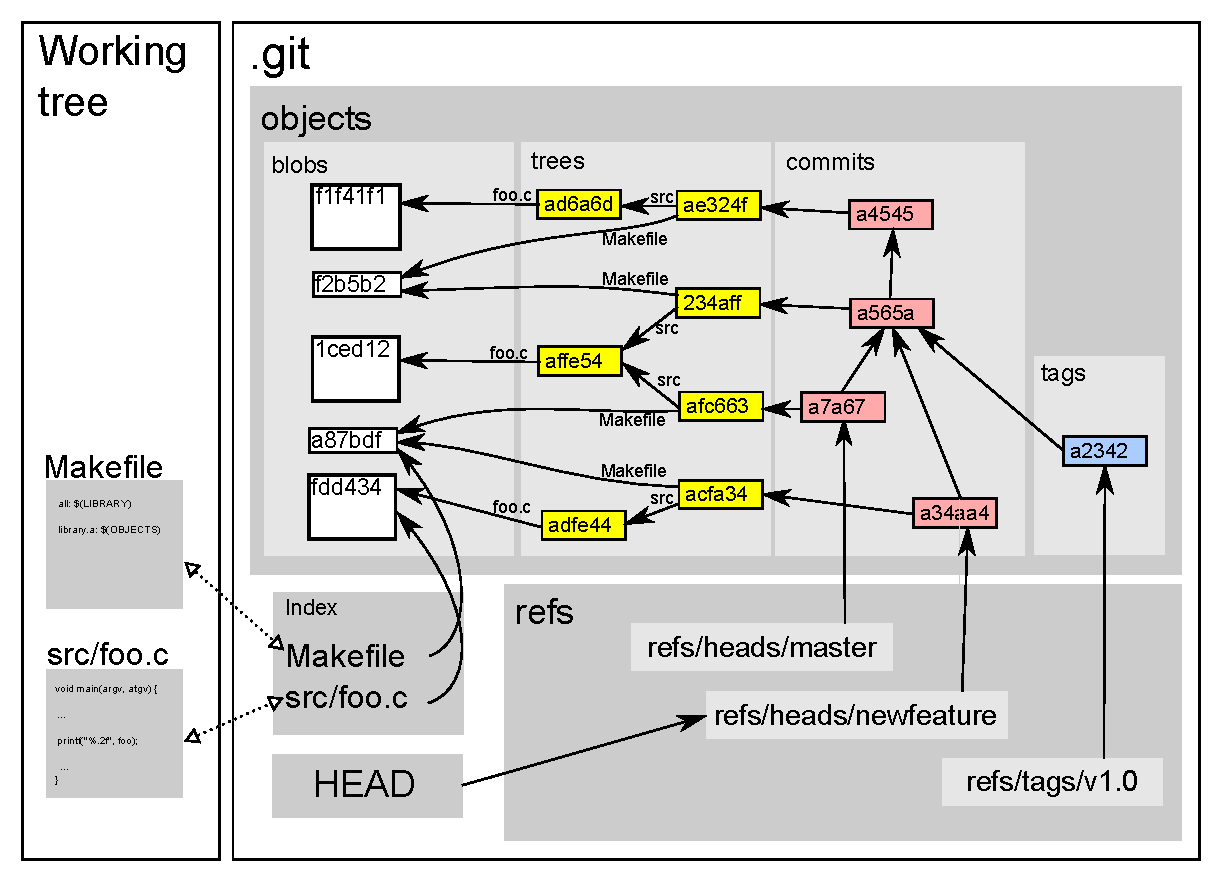
\includegraphics[height=70mm]{git_object_database.pdf}
        \mode<article>{
          \caption{Internal structure of a Git repository}
          \label{fig:objectdatabase}
        }%
      \end{center}
    \end{figure}
  }

\end{frame}

\begin{frame}[fragile]
  \frametitle{Git object database}

  \mode<article>{

    The actual data of a Git repository, such as the history and the
    contents of the files, is entirely stored in the Git object
    database. This database is a simple Document-oriented database
    that indexes the objects by the SHA1 checksum of the contents.

    This has a few very important consequences:

    \begin{itemize}

      \item It is very easy to perform consistency checking on the
        database data. You know that the name of the object should
        \emph{always} be the SHA1 checksum of its contents.

      \item Objects are automatically unique by their content, if you
        try to create another object with the same contents you will
        always end up with the same SHA1 checksum, which means you
        will never have duplicate objects in the database.

      \item Objects are always read-only, since changing the contents
        of an object necessarily means you have a different checksum
	an therefore a different name.

      \item It is generally considered to not be feasible to
        craft a different content that results in the same SHA1
        checksum, and even if that is at all possible, it is even
        harder to craft a file that resembles a legitimate file.

    \end{itemize}

    There are four different types of objects that can be stored in
    the Git object database:

    \begin{enumerate}
      \item[blob]{Blobs are just raw contents of data. They are used
        to represent the contents of the files in your repository.}
      \item[tree]{A tree is how Git represents a ``directory''.
	It stores pointers to blobs (files) and other trees
	(directories).  Each of these pointers had a name, file
	mode, etc. (much like an inode in the Unix filesystem).
	The pointer is just its name, a SHA1 checksum.}
      \item[commit]{A commit represents one particular state of the
        repository. It points to the tree that represents the root
        directory and to zero, one or more parent commits,
        representing which states where used as starting point for
        this particular state. The initial commit in a repository has
        no parents, most commits have one parent and the merge commits
        have two or more parents. The commit object also stores
	information about when and who committed this version and
	the associated commit message.}
      \item[tag]{A tag object, also known as an ``annotated tag'', is an
        object that points to a commit and also holds additional
        metadata, such as the date, the name of the person creating
        the tag, some comments, and possibly a PGP/GPG digital
        signature.}
    \end{enumerate}

    Note that as Figure ~\ref{fig:objectdatabase} shows, the set of
    objects make a Directed Acyclic Graph: The commit points to the
    earlier commits and to the tree, the tree points to tress and
    blobs.

    }


\defverbatim[colored]\screensession{%
\begin{lstlisting}
>> find .git/objects -type f | head -5
.git/objects/ab/f8749fabd64057bde7f28fce0a3cfbb8c998d2
.git/objects/3f/a50dd375ea568c11bcf20bca23f47f9c27186e
.git/objects/bc/dce3cae827b2c0074ca8319bad04a10149dffa
.git/objects/cf/c1e8c3a035b59819fef4fb70e7aed6ed0cca24
.git/objects/ee/619d614c790a93546a94e36b8ca36f9d80e56e
\end{lstlisting}
}

  \mode<presentation>{
  \only<2>{
    \begin{itemize}
    \item Four types: blobs, trees, commits and tags
    \item SHA1 indexed
    \item Cryptographic security
    \item Directory structure:\\
      \screensession
    \end{itemize}
  }
  }

  \mode<article>{

    What might not seem so obvious is the consequence of using SHA1
    checksum object ids and a Directed Acyclic Graph at the same
    time. Let me go through so it is made as clear as possible:

    \begin{itemize}
      \item The contents of the files in the repository are used to
        generate the object ids, you can easily check if the object is
        consistent, as illustrated earlier.
      \item A tree object contains references to the object ids of the
        blobs it references, being also an object, the tree itself is
        checksummed to produce its object id.
      \item When a tree contains other trees, it again references to
        SHA1 ids of the subtrees and is itself indexed by its
        checksum.
      \item Finally, the commit will have in its contents the object
        id for the tree object that contains the root directory as
        well as the id of the parent commit. A commit being an object
        itself also is checksummed to produce its id.
      \item A tag, finally, points to the sha1 checksum object id of a
        commit file and is, itself, checksummed to produce the object
        id.
    \end{itemize}

    The result is that, in order to authenticate a given revision of
    the repository, you only need to authenticate the topmost object
    of the graph (i.e.: a tag). Once you authenticate the tag, since
    it recursively is the product of the checksum of all the contents
    in the repository, you can trust the authenticity of the entire
    history of the repository.

    Git provides tools to use GPG/PGP to digitally sign tags, but any
    authenticated message that lists a commit id is sufficient to make
    the entire history and contents behind that commit trusted.

  }


\defverbatim[colored]\screensession{%
\begin{lstlisting}
>> git log --oneline -n1
b35f7bd fixed some bugs in the interface
>> git cat-file -p b35f7bd
tree 79200d4e812c1b2566c324562b243449f1a23841
parent aecd06b8d666b901b2a0cb53a947462d7dcb8bcb
author John Doe <john@foobar.net> 1305056906 -0400
committer John Doe <john@foobar.net> 1305056906 -0400
>> git cat-file -p 79200d4e
040000 tree a14bb0feff3cd4ece851336efc0c2cf8bed94e83    src
100644 blob 264321f3b12812d443ebedf19b6a63787a58a760    Makefile
\end{lstlisting}
}

  \only<3>{
    Looking at objects used in a commit
    \screensession
  }

\end{frame}

\begin{frame}[fragile]
  \frametitle{References}

  \mode<article>{

    We mentioned references earlier when we were talking about
    branches. Branches are just one specific type of reference, and,
    in fact, the difference between branches and other
    references\footnote{You will see the name ``references'' being
      abbreviated as ``refs'' in the Git documentation} happens only
    in the commands that operate at the high level -- the layer
    above the database. For the Git object database per se, there
    is no distinction between the references.

    All refs are simply pointers to objects (e.g., commits or
    tags) or sometimes to other refs. You can see them in your
    repository by doing a simple:

  }

\defverbatim[colored]\screensession{%
\begin{lstlisting}
>> find .git/refs -type f
.git/refs/heads/master
.git/refs/remotes/origin/HEAD
.git/refs/remotes/origin/master
>> cat .git/refs/heads/master
fcebb0e265b728486b8cbac88bb35af34d9efa15
>> cat .git/refs/remotes/origin/master
fcebb0e265b728486b8cbac88bb35af34d9efa15
\end{lstlisting}
}

  \only<2>{
    \mode<presentation>{
      \begin{itemize}
      \item A named pointer (e.g., to a commit or tag)
      \end{itemize}
    }
    \screensession
  }
\end{frame}

The references are primarily used to keep track of branches (both local
and remote) and tags. But other tools that are part of Git or that use
Git make extensive use of references. For instance, the ``notes''
command uses refs to store information annotating existing commits.

\begin{frame}[fragile]
  \frametitle{The index}
  \only<2>{
    \begin{itemize}
    \item A single file
    \item Links to all staged files (blobs)
    \item Like a tree, but multilevel
    \end{itemize}
  }
\end{frame}

The purpose of the index was mentioned before, so here we will just
cover the technical aspects. The index is the equivalent of a fully
recursive tree that represents the version that was initially
populated in your working directory.

When you add a new file or a new version of an existing file to the
index, the blob object is created with the entire contents of the new
version and this new blob is referenced by the index.

When you do the commit, it won't need to perform the SHA1 checksum of
the changed files, since that was done at the moment you did the
\texttt{add}. And that's why the \texttt{commit} operation usually is
faster then the \texttt{add} operation (specially if you changed a lot
of files).

\begin{frame}[fragile]
  \frametitle{The HEAD}

  \only<2>{
    \begin{itemize}
    \item A pointer to the current branch, commit, etc.
    \item Branches are moved by commit, tags are not
    \item You should probably always work on a branch
    \end{itemize}
  }

  \mode<article>{

    The HEAD represents your current point in the history (the
    commit that you checked out).  It is like a ref, but
    technically isn't because it is not in the \texttt{.git/refs/}
    directory.  It is used by the commit operation to find the
    ``parent'' of the new commit and also to update the ref when
    you are in a branch.

    The way this works is that Git honors ``symbolic references''.
    When the HEAD contains a symbolic reference, it points to the
    branch that was checked out, not directly to the commit.  This
    way the commit command knows which branch ref to update.
    
    The following snippet shows that when you checkout a branch, you
    get a symbolic reference in the HEAD, which means Git will work as
    you normally expect. But if you checkout anything else (for
    example, a tag), HEAD will contain a SHA1 and
    you will be in the ``Detached HEAD'' state, which means that,
    upon commit, Git will only update the HEAD, but no reference will
    point to the new commit.

  }

\defverbatim[colored]\screensession{%
\begin{lstlisting}
>> git checkout master
>> cat .git/HEAD
ref: refs/heads/master
>> git checkout v1.2tag
>> cat .git/HEAD
ab99e4e669177cde4ea9ae930974675310ba2cb3
>> git checkout -b v1.2.1branch v1.2tag
>> cat .git/HEAD
ref: refs/heads/v1.2.1branch
\end{lstlisting}
}

  \only<3>{%
    \screensession
  }

\end{frame}

\againframe<1,3>{architecture}


\end{document}
